\documentclass[xcolor=dvipsnames]{beamer}
%\usetheme[progressbar=frametitle]{metropolis}
\usecolortheme{seahorse}

\definecolor{gray}{HTML}{151515}
\definecolor{orange}{HTML}{d28445}

\setbeamercolor{normal text}{fg=gray}
\setbeamercolor{progress bar}{fg=orange}

% balíčky

\usepackage[utf8]{inputenc}
\usepackage[czech]{babel}
\usepackage{graphicx, tabularx}
\usepackage{amsmath, amssymb, amsthm}
\usepackage{subcaption, wrapfig}
\newcommand{\abs}[1]{\lvert #1 \,\rvert} %}}}
\usefonttheme[onlymath]{serif}	
\usepackage{dashrule}

%gets rid of bottom navigation bars
\setbeamertemplate{footline}[frame number]

%gets rid of bottom navigation symbols
\setbeamertemplate{navigation symbols}{}

%gets rid of footer
%will override 'frame number' instruction above
%comment out to revert to previous/default definitions
% \setbeamertemplate{footline}{} 

\usepackage{asymptote}
\usepackage{epstopdf}
\usepackage{xcolor}

\usepackage[backend=biber, url=true, sorting=none]{biblatex}
\renewcommand*{\bibfont}{\footnotesize}
\addbibresource{/home/adam/tex/soc.bib}
\usepackage{url}

\title{Mechanika rodin planetek \\ s aplikací na rodinu Eunomia}
\author{Adam Křivka \\ \and doc. Mgr. Miroslav Brož, Ph.\,D.}
\institute{Cyrilometodějské gymnázium a střední odborná škola pedagogická Brno,\\ Lerchova 63, 602 00 Brno}

\begin{document}

{
\setbeamerfont{title}{shape=\bfseries}
\setbeamerfont{author}{shape=\bfseries}
\setbeamercolor{author}{fg=white}
\setbeamerfont{institute}{shape=\bfseries}
\setbeamercolor{institute}{fg=white}
\setbeamerfont{date}{shape=\bfseries}
\setbeamercolor{date}{fg=white}
\setbeamertemplate{frametitle}{}
\setbeamertemplate{title}{}
\usebackgroundtemplate{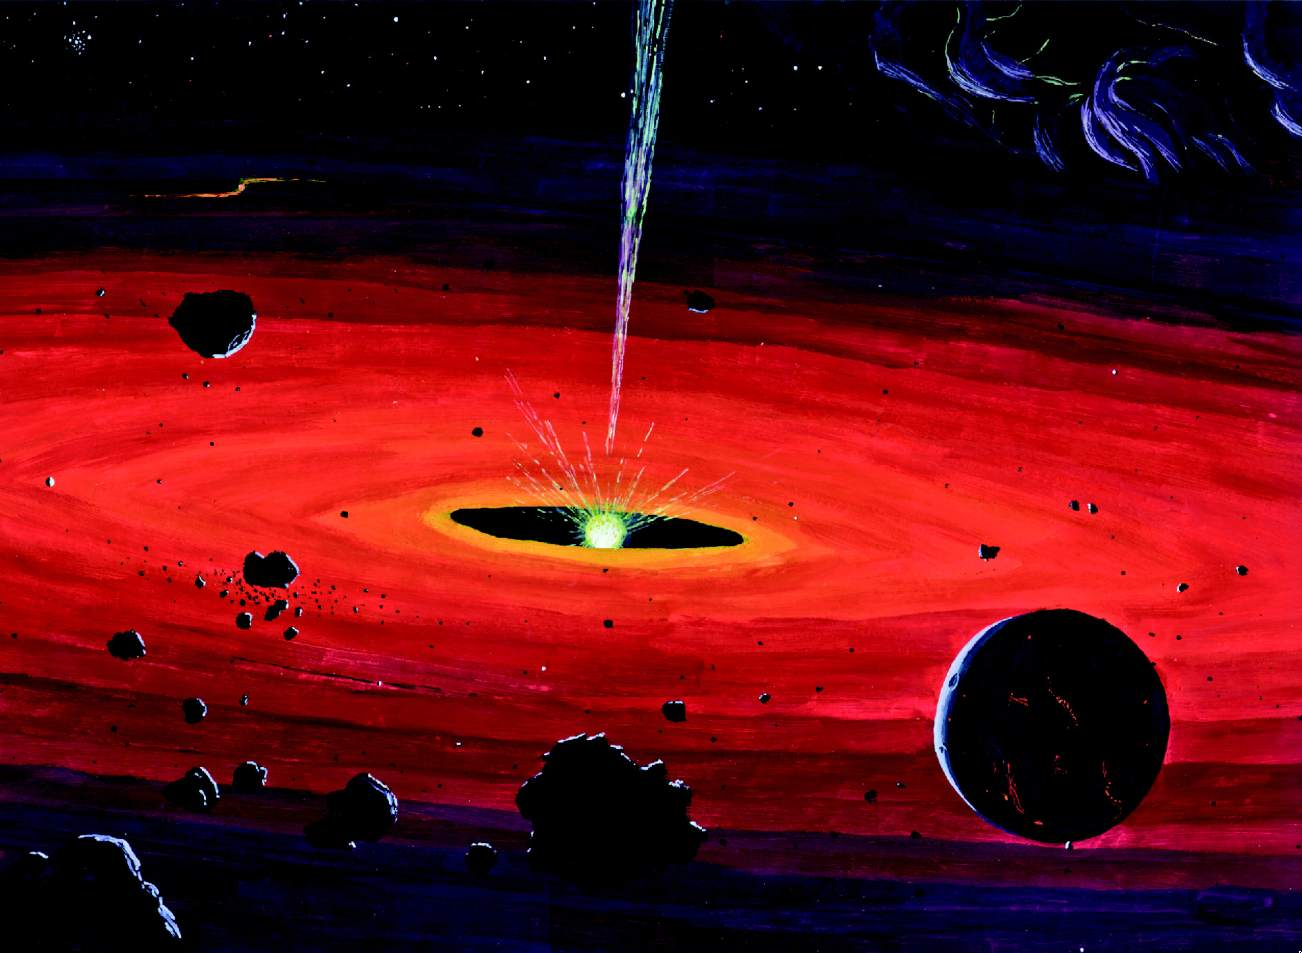
\includegraphics[height=\paperheight]{../obr/fmt.jpg}}%

\begin{frame}[t]
	\titlepage
\end{frame}
}

\begin{frame}{Struktura}
	\textcolor{white}{\tableofcontents}
\end{frame}


\section{Úvod}


\begin{frame}[t]{\secname}{Historický pohled a význam}
	\begin{itemize}
		\item První planetka byla objevena v roce 1801.
		\item Dnes známo již přes půl milionu planetek.
		\item Rodiny planetek poprvé studoval \textit{Kiyotsugu Hirayama} (1874--1943).
		\item[!] \textit{Správné české označení je planetka, nikoliv asteroid.} 
		\end{itemize}
	\vfill
	\begin{itemize}
		\item Studiem rodin planetek můžeme 
		\begin{itemize}
			\item pochopit \textbf{dynamickou strukturu} sluneční soustavy,
			\item podpořit teorie o \textbf{vzniku sluneční soustavy} (např. \textit{Velké pozdní bombardování})
		\end{itemize}
	\end{itemize}
\end{frame}


\section{Planetky ve sluneční soustavě}


\begin{frame}[t]{\secname}{Tvar a vznik}
	\begin{figure}
		\centering
		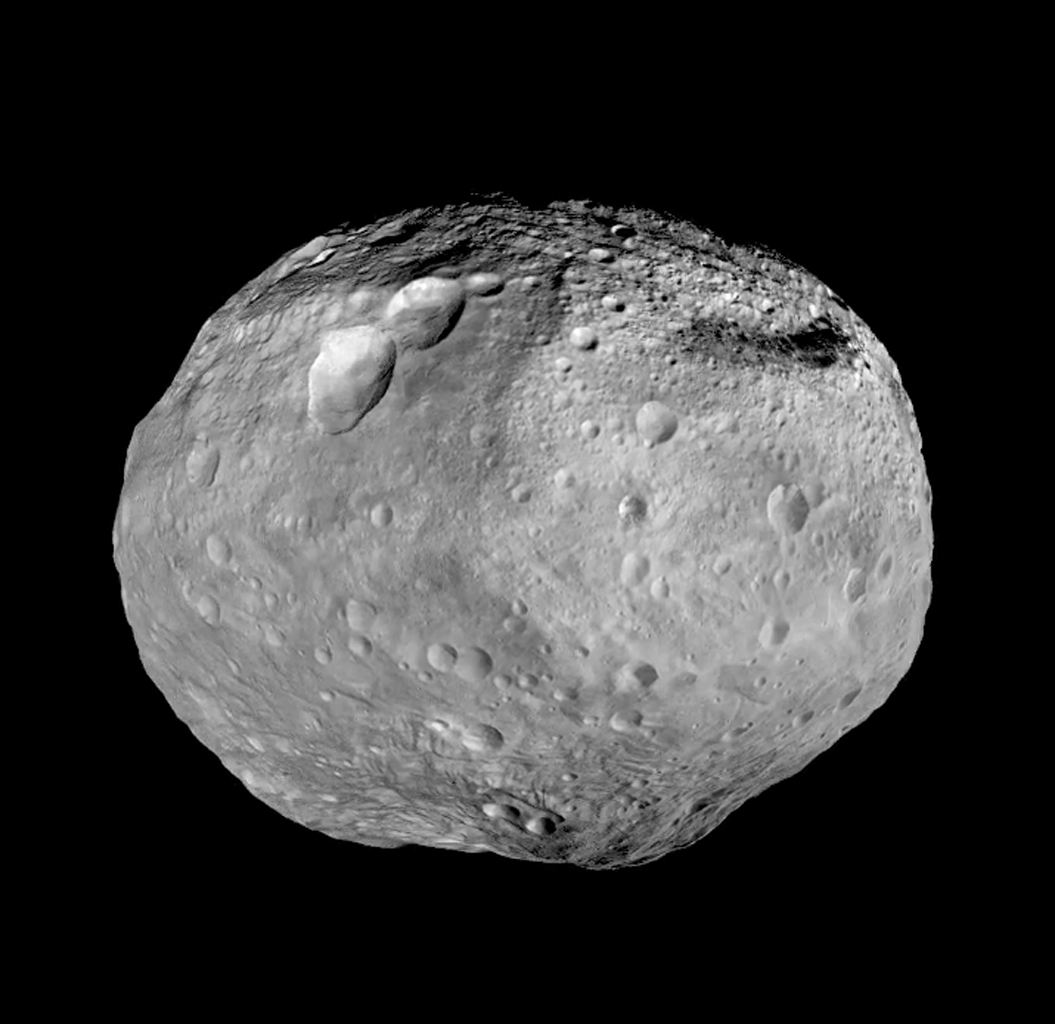
\includegraphics[height=0.65\textheight,width=\textwidth,keepaspectratio]{../obr/vesta.jpg}
		\caption{\footnotesize{Planetka \textit{(4) Vesta}. Fotografie byla pořízena americkou sondou \textit{Dawn}. Převzato z~\cite{jplvesta}.}}
	\end{figure}
\end{frame}

\begin{frame}[t]{\secname}{Rodiny planetek}
	\begin{figure}
		\centering
		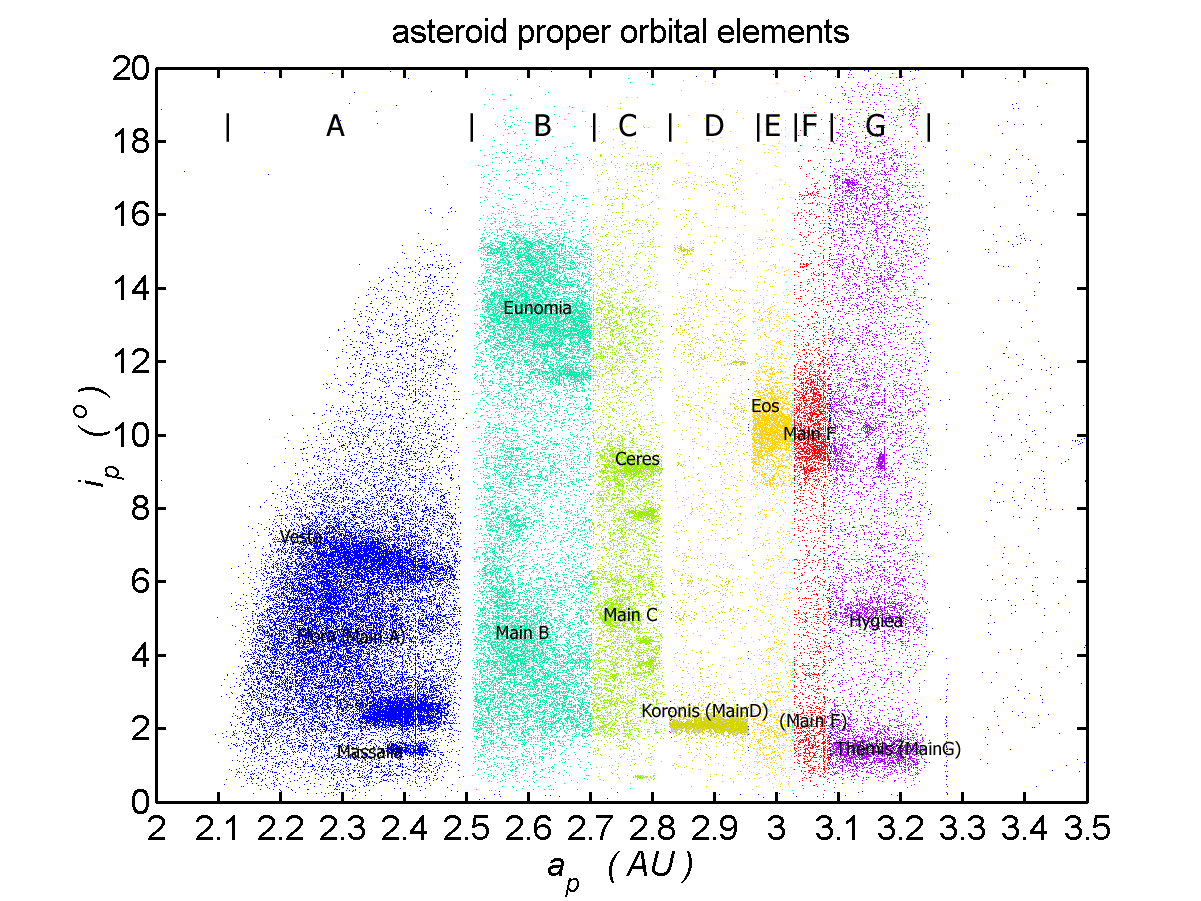
\includegraphics[height=0.65\textheight,width=\textwidth,keepaspectratio]{../obr/mainbelt.png}
		\caption{\footnotesize{Planetky \textbf{hlavního pásu} podle \textbf{vlastních elementů dráhy} --- vlastní velké poloosy $a_{\rm p}$ a vlastního sklonu $i_{\rm p}$. Převzato z~\cite{wiki:belt}.}}
	\end{figure}
\end{frame}

\begin{frame}[t]{\secname}{Negravitační perturbace}
\begin{itemize}
\item Jarkovského jev

\begin{figure}
\centering
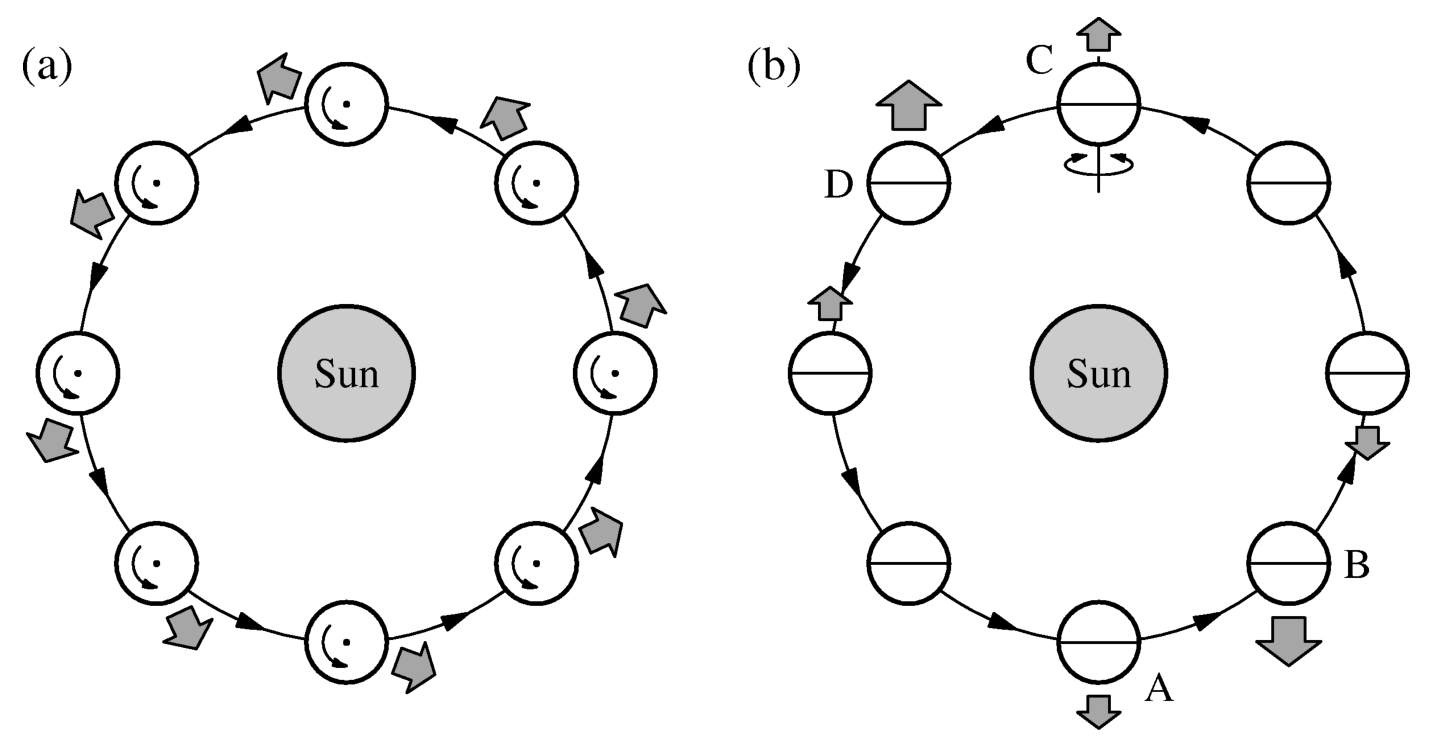
\includegraphics[width=0.6\textwidth]{../obr/jarkovskeho_jev.png}
\end{figure}

\item YORP jev
\item Náhodné srážky
\item Chaotická difuze
\end{itemize}

\end{frame}


\section{Nebeská mechanika}


\begin{frame}[t]{\secname}{Elementy dráhy}
	\begin{columns}
		\begin{column}{0.5\textwidth}
		\begin{itemize}
			\item \textbf{Velká poloosa} $a\,[{\rm AU}]$  
			\item \textbf{Excentricita} $e$
			\item \textbf{Sklon} $i\,[ ^\circ]$
			\item Argument pericentra $\omega\,[ ^\circ]$
			\item Délka vzestupného uzlu $\Omega\,[ ^\circ]$
			\item Střední anomálie $M \,[ ^\circ]$
		\end{itemize}
		\end{column}
		\begin{column}{0.5\textwidth}
			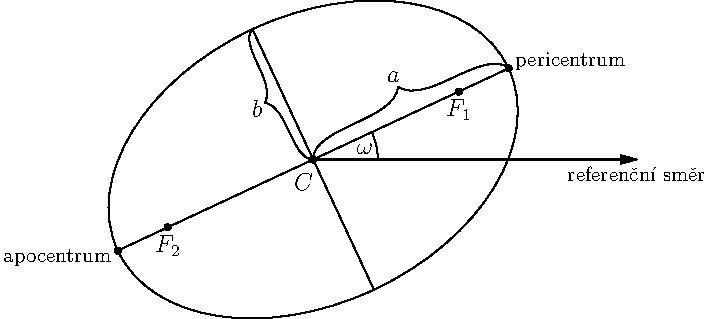
\includegraphics[width=1.1\textwidth]{../asy/asteroidy-1.pdf}
			\
			\begin{align*}
				e=\sqrt{1-\frac{b^2}{a^2}}
			\end{align*}
		\end{column}
	\end{columns}
\end{frame}

\begin{frame}[t]{\secname}{Střední a vlastní elementy}
	\begin{figure}
		\centering
		\begin{subfigure}[b]{0.49\textwidth}
		\centering
		\includegraphics[width=1.0\textwidth]{../obr/atOF}
		\end{subfigure}
		\begin{subfigure}[b]{0.49\textwidth}
		\centering
		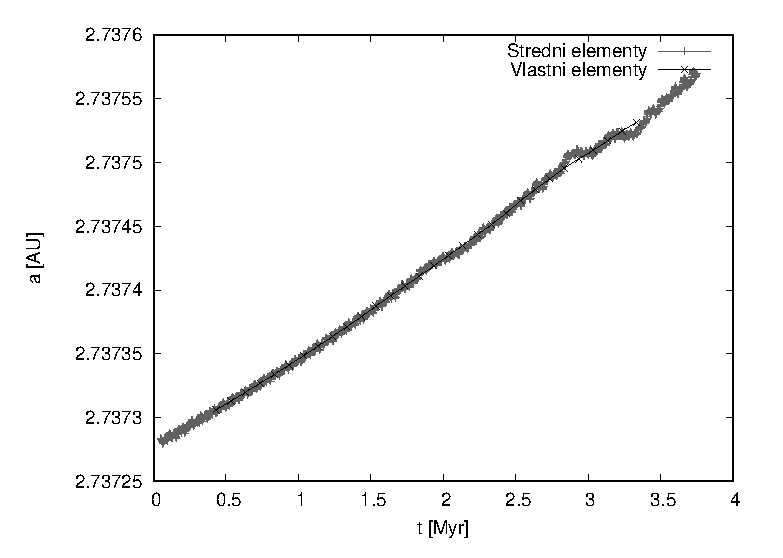
\includegraphics[width=1.0\textwidth]{../obr/atFP}
		\end{subfigure}
		\caption{\ Porovnání \textbf{oskulační} (aktuální) a \textbf{střední} hlavní poloosy (vlevo) a \textbf{střední} a~\textbf{vlastní} hlavní poloosy (vpravo) pro simulaci jedné částice po dobu $3,76$ miliónů let.}
	\end{figure}
\end{frame}

\begin{frame}[t]{\secname}{Problém $N$ těles}
	\begin{figure}
		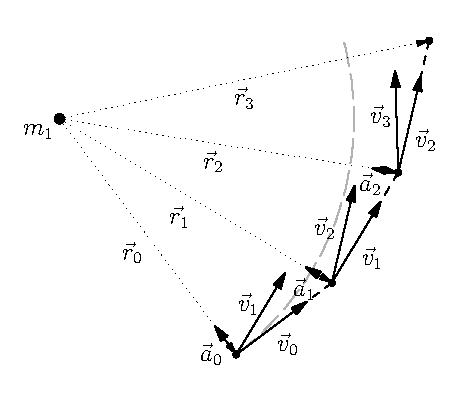
\includegraphics[width=0.49\textwidth]{../asy/asteroidy-3.pdf}
		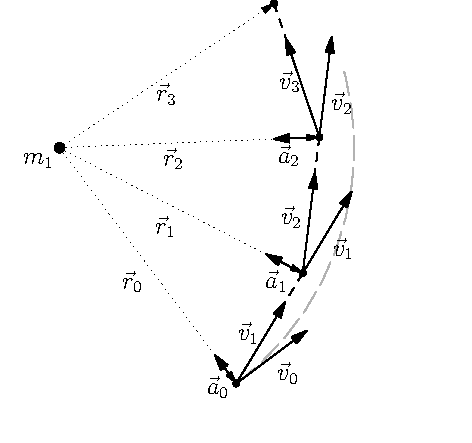
\includegraphics[width=0.49\textwidth]{../asy/asteroidy-4.pdf}
		\vspace{-1cm}
		\caption{\footnotesize{Ilustrace dopředné (vlevo) a zpětné (vpravo) \textbf{Eulerovy metody} pro výpočet problému dvou těles.}}
	\end{figure}
	\vspace{-0.5cm}
	\begin{align*}
		m_i\vec{a}_i &= -\sum_{\substack{j=1 \\ j\neq i}}^N \frac{Gm_im_j}{\abs{\vec{r}_i-\vec{r}_j}^3}(\vec{r_i}-\vec{r_j})\,, \qquad{\rm pro}\ i\in\{1,\,2,\,\dots,\,N\} \label{eq:nbody2}
	\end{align*}
\end{frame}

% \begin{frame}[t]{\secname}{Krátkodobé simulace}
% \begin{figure}
% 	\centering
% 	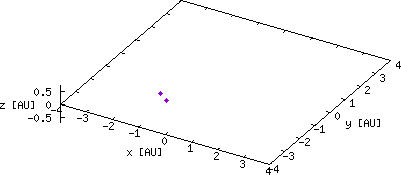
\includegraphics[width=0.49\textwidth]{../obr/trajec_001t.png}
% 	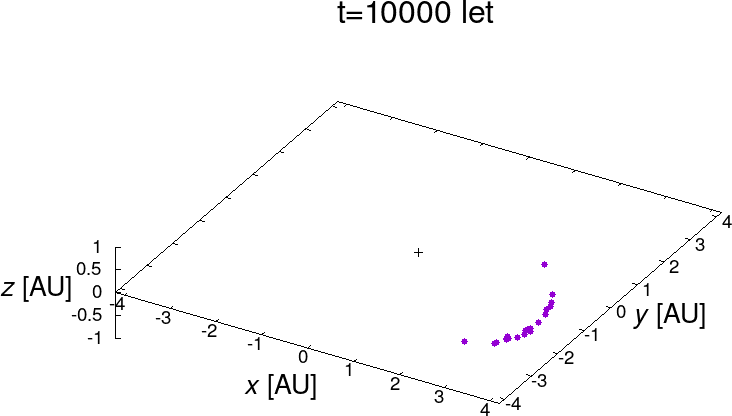
\includegraphics[width=0.49\textwidth]{../obr/trajec_101t.png} \\
% 	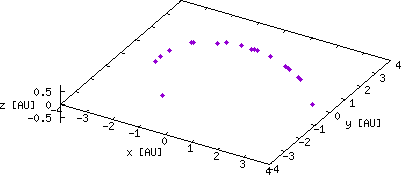
\includegraphics[width=0.49\textwidth]{../obr/trajec_201t.png}
% 	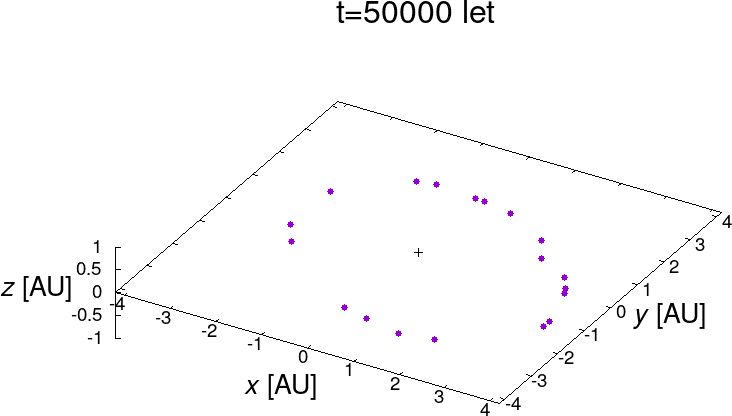
\includegraphics[width=0.49\textwidth]{../obr/trajec_501t.png}
% 	\caption{\textbf{Trojrozměrné polohy} $x,\,y,\,z$ několika těles ($N=20$) ze \textbf{simulované} rodiny Eunomia \textbf{rušené} čtyřmi planetami (\textit{Jupiterem}, \textit{Saturnem}, \textit{Uranem} a~\textit{Neptunem}) po úvodním \textbf{izotropním} rozpadu.} \label{fig:trajec}
% \end{figure}
% \end{frame}


\section{Vlastnosti rodiny Eunomia}


\begin{frame}[t]{\secname}{Identifikace členů}
	\vspace{-1cm}
	\begin{figure}
		\centering
		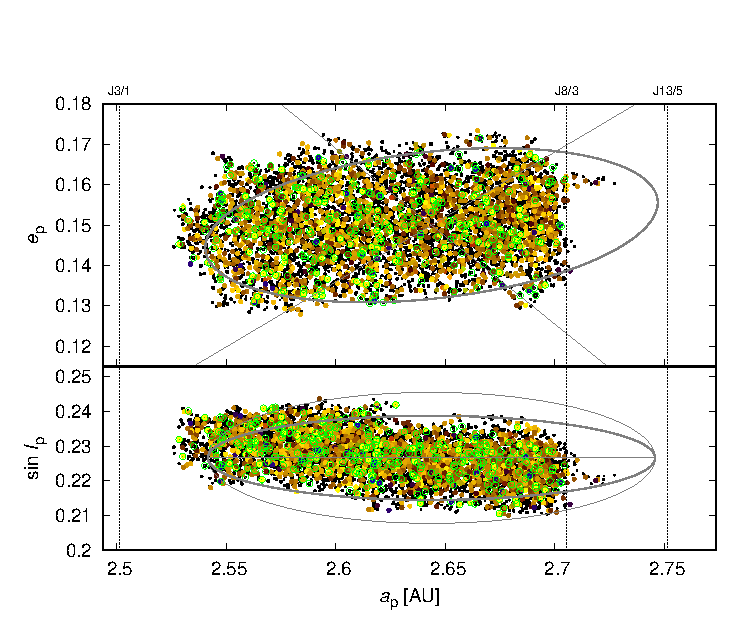
\includegraphics[width=0.8\textwidth]{../obr/ae_ai_wise}
		\vspace{-0.3cm}
		\caption{\footnotesize{\textbf{Pozorovaná} rodina Eunomia v~rovině vlastní hlavní poloosy $a_{\rm p}$ a vlastní excentricity $e_{\rm p}$, identifikovaná \textbf{hierarchickou shlukovací metodou}. Barevná škála odpovídá \textbf{albedu} $p_{\rm V}$ a $p_{\rm IR}$ z~katalogu WISE\@.}}
	\end{figure}
\end{frame}

\begin{frame}[t]{\secname}{Barevné charakteristiky}
	\begin{figure}
	\captionsetup[subfigure]{justification=centering}
		\begin{subfigure}[c]{0.49\textwidth}
			\centering
			\includegraphics[width=1.0\textwidth]{../obr/pV_pIR-crop}
			\caption{\textbf{Albeda} $p_{\rm V}$ (ve viditelném spektru) a~$p_{\rm IR}$ (v~infračerveném) z~katalogu WISE. Pro vyřazení \textbf{přimísených těles} byly zvoleny hraniční hodnoty $0,05 \leq p_{\rm V} \leq 0,4$.}
		\end{subfigure}
		\begin{subfigure}[c]{0.49\textwidth}
			\centering
			\includegraphics[width=1.0\textwidth]{../obr/astar_iz-crop}
			\caption{\textbf{Barevné indexy} $a^*$ a~$i-z$ z~katalogu Sloan. Pro vyřazení \textbf{přimísených těles} byly zvoleny hraniční hodnoty $0\leq a^* \leq 0,3$ a~$-0,3\leq i-z \leq 0,3$.}
		\end{subfigure}

	\end{figure}
\end{frame}

\begin{frame}[t]{\secname}{Jarkovského a YORP jev}
	\begin{figure}
		\centering
		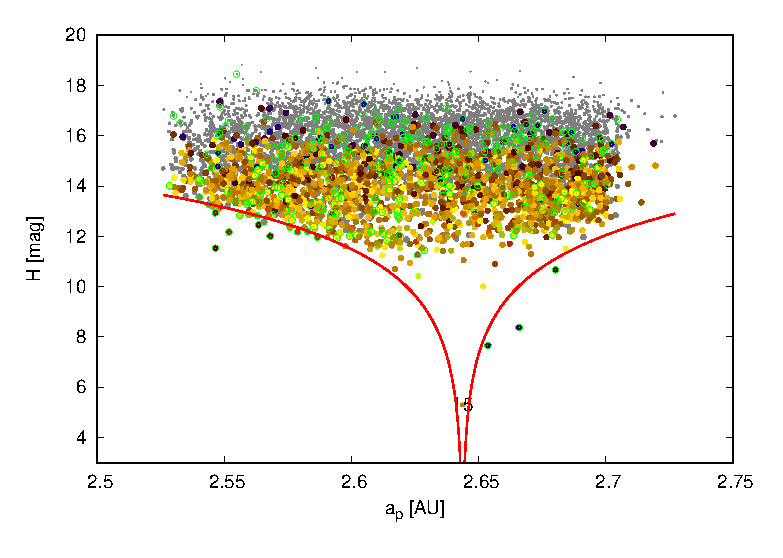
\includegraphics[width=0.7\textwidth]{../obr/aH_wise.eps}
		\caption{\footnotesize{Rozdělení pozorované rodiny \textit{Eunomia} v~rovině vlastní hlavní poloosy $a_{\rm p}$ a \textbf{absolutní hvězdné velikosti} $H$. Lze pozorovat typický tvar \uv{V}, který je způsobem počátečním rychlostním polem a \textbf{Jarkovského jevem}.}}
	\end{figure}
\end{frame}


\begin{frame}[t]{\secname}{Nastavení simulace}
	\begin{columns}
	\begin{column}{0.6\textwidth}
		\begin{itemize}
			\item 6210 vzájemně \textbf{gravitačně neinteragujících} částic, 4 rušící planety (\textit{Jupiter}, \textit{Saturn}, \textit{Uran}, \textit{Neptun})
			\item \textbf{Numerický integrátor} SWIFT (vhodný pro dlouhodobé simulace)
			\item Délka úspěšného bloku 500 miliónů let
			\item \textit{Výpočetní cluster Astronomického ústavu Univerzity Karlovy}
			\begin{itemize}
				\item Spotřebováno 23040 CPU hodin
				\item Objem binární dat $164\,{\rm GB}$ 
			\end{itemize}
		\end{itemize}
	\end{column}
	\begin{column}{0.4\textwidth}
		\begin{figure}
			\centering
			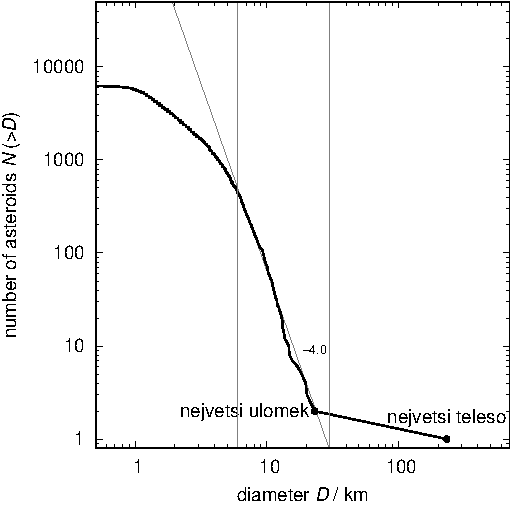
\includegraphics[width=1\textwidth]{../obr/size_distribution-crop}
			\caption{\textbf{Histogram} četnosti velikostí planetek rodiny \textit{Eunomia}.}
		\end{figure}
	\end{column}
	\end{columns}
\end{frame}

\begin{frame}[t]{\secname}{Výsledky simulace}
	\centering
	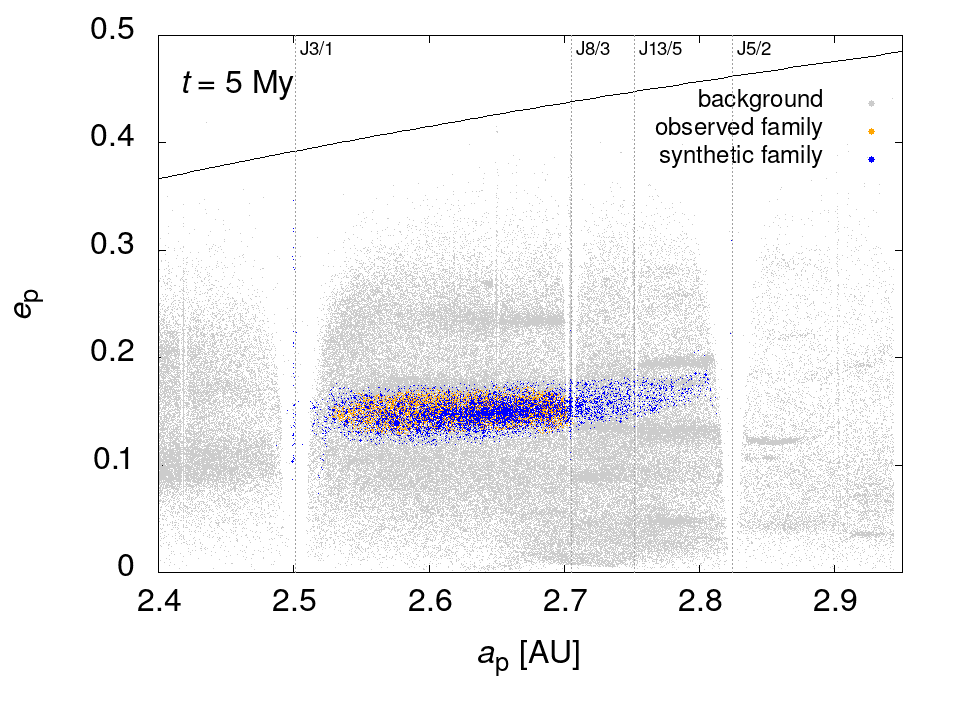
\includegraphics[width=0.8\paperwidth]{../obr/ae_5_trans.png}
\end{frame}

\begin{frame}[t]{\secname}{Metoda blackbox (chí kvadrát)}
	\begin{itemize}
		\item Rozdělení těles do \textbf{boxů}

		\begin{table}
		\centering
{\footnotesize
			\begin{tabularx}{0.9\textwidth}{|X||c|c|c|}
				\hline
				& Spodní mez & Horní mez & Velikost  \\
				\hline \hline
				Vlastní hlavní poloosa $a_{\rm p}$ & $2,522\,{\rm AU}$ & $2,844\,{\rm AU}$ & $0,0153\,{\rm AU}$ \\
				\hline
				Vlastní excentricita $e_{\rm p}$ & $0,1$ & $0,23$ & $0,0217$ \\
				\hline
				Vlastní sklon $\sin I_{\rm p}$ & $0,2$ & $0,25$ & $0,05$ \\
				\hline
			\end{tabularx}
}
		\end{table}

		\item Použita statistická metoda \textbf{chí kvadrátu}
		\begin{itemize}
			\item Příspěvek každého boxu se spočte jako
			\begin{align*}
				\frac{(N_{\rm sim}-N_{\rm obs})^2}{N_{\rm sim}+N_{\rm obs}}
			\end{align*}
			\item Celková hodnota $\chi^2$ se spočte jako součet přes všechny boxy	
		\end{itemize}
	\end{itemize}
\end{frame}

\begin{frame}[t]{\secname}{Analýza chí kvadrátu}
	\centering
	\begin{figure}
		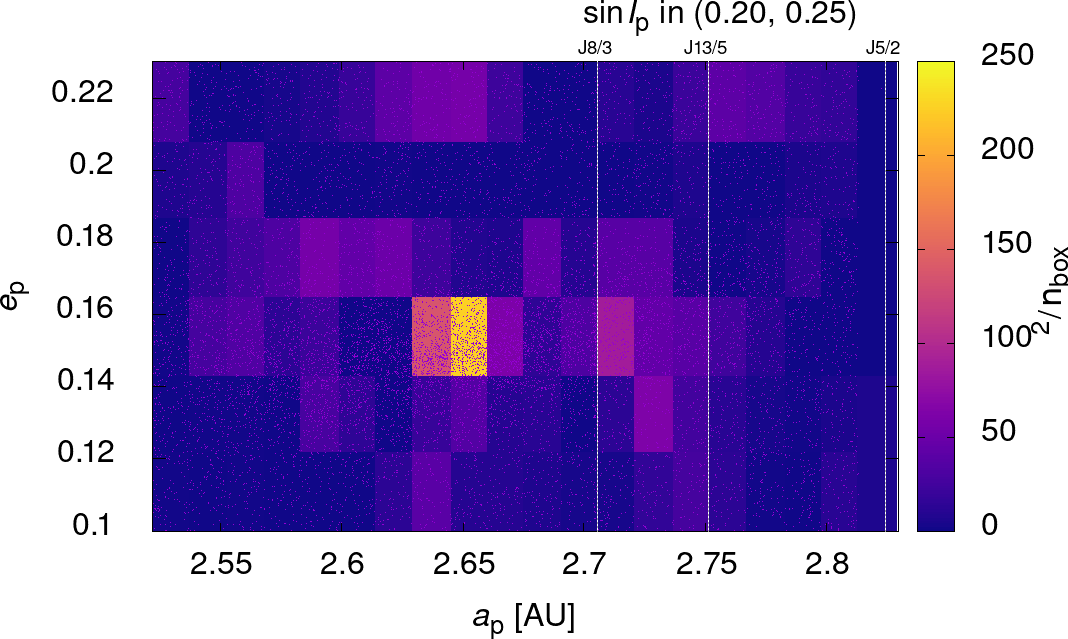
\includegraphics[width=0.41\paperwidth]{../obr/ae_chi_0006t.png}
		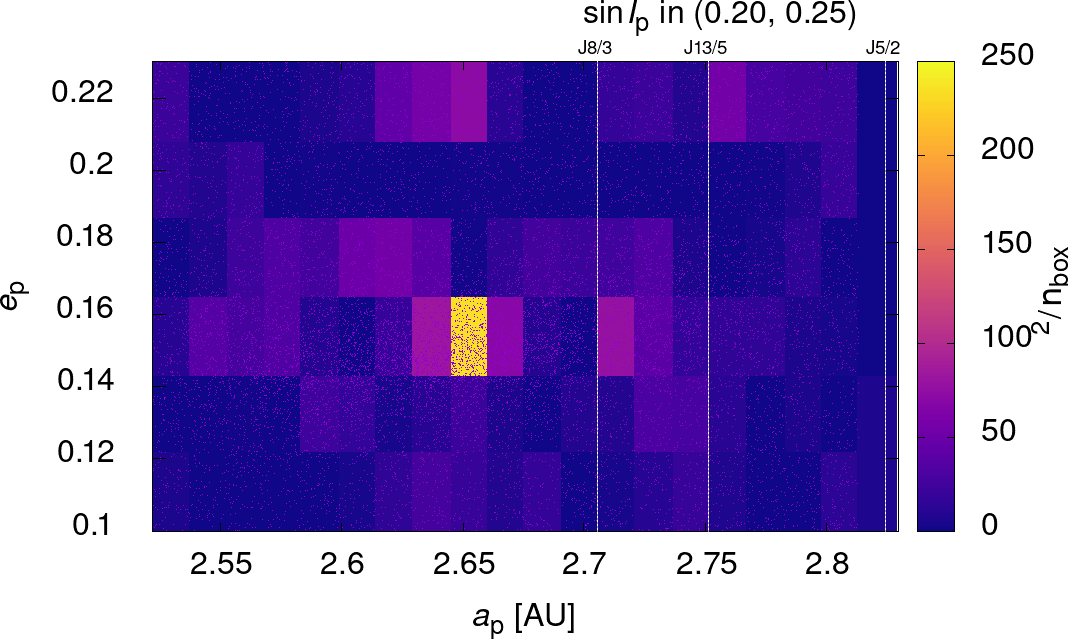
\includegraphics[width=0.41\paperwidth]{../obr/ae_chi_0106t.png}\\
		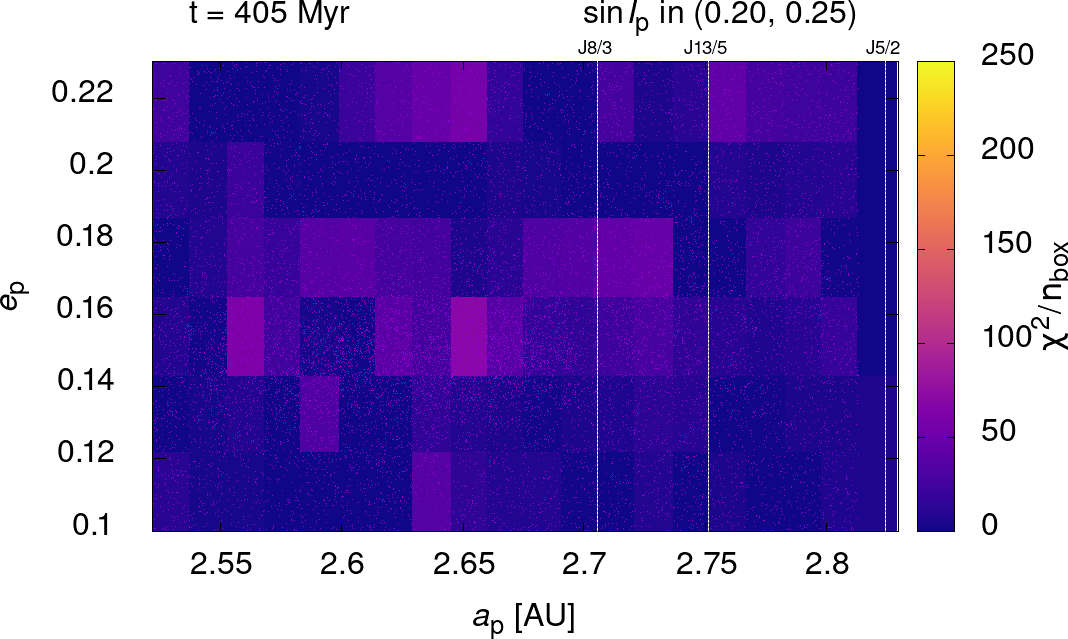
\includegraphics[width=0.41\paperwidth]{../obr/ae_chi_0406t.png}
		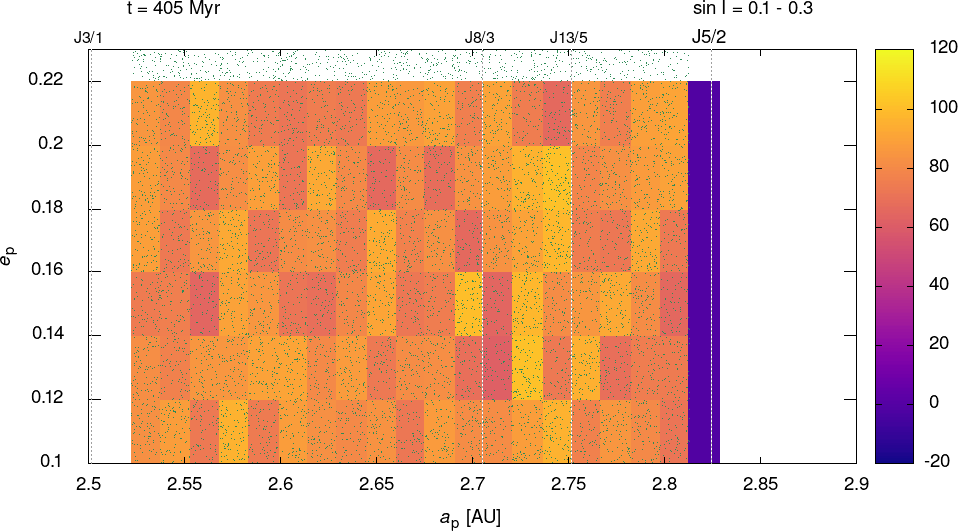
\includegraphics[width=0.41\paperwidth]{../obr/ae_chi_emptyt.png}

		\caption{Hodnota \textbf{chí kvadrátu} $\chi^2$ pro každý \textbf{box} v~prostoru $(a_{\rm p},\,e_{\rm p})$.} \label{fig:ae_chi2}
	\end{figure}

\end{frame}

\begin{frame}[t]{\secname}{Porovnání simulované a pozorované rodiny}
	\newcolumntype{V}{>{\centering\arraybackslash} m{.4\linewidth} }
	\begin{tabularx}{\textwidth}{c V}
		\centering
		Simulovaná: & \includegraphics[width=0.46\paperwidth]{../obr/ae_scl.png}\\
		Pozorovaná: & \includegraphics[width=0.46\paperwidth]{../obr/ae_obs.png}
	\end{tabularx}
\end{frame}


\section{Závěr}


\begin{frame}[t]{\secname}{Výsledky}
	\begin{itemize}
	\item Několik krátkodobých simulací %(např. k ukázce středních a vlastních elementů)
	\item Identifikace členů rodiny Eunomia
	\item Úspěšná simulace orbitálního vývoje rodiny Eunomia
	\item Popis dynamické struktury rodiny Eunomia
	\item Odhad stáří rodiny Eunomia na pravděpodobně více než 500 miliónů let
	\end{itemize}
\end{frame}

\begin{frame}[c]{\secname}{Budoucí práce}
	\begin{figure}
		\centering
		\large \textit{Ten \uv{positivní} graf}
		\includegraphics[width=0.7\textwidth]{../obr/chi2}
		\caption{Graf závislosti hodnoty \textbf{chí kvadrátu} na čase $t$.}
	\end{figure}
\end{frame}

\begin{frame}[t]{\secname}{Reference a doporučená literatura}
	\printbibliography

	{\color{blue}\hdashrule[0.5ex]{\textwidth}{0.7pt}{2mm}}

	\newrefsection{}
	\setbeamertemplate{bibliography item}[book]
	\nocite{fmt}
	\nocite{murray00}
	\nocite{brozphd}
	\printbibliography
\end{frame}

{
\usebackgroundtemplate{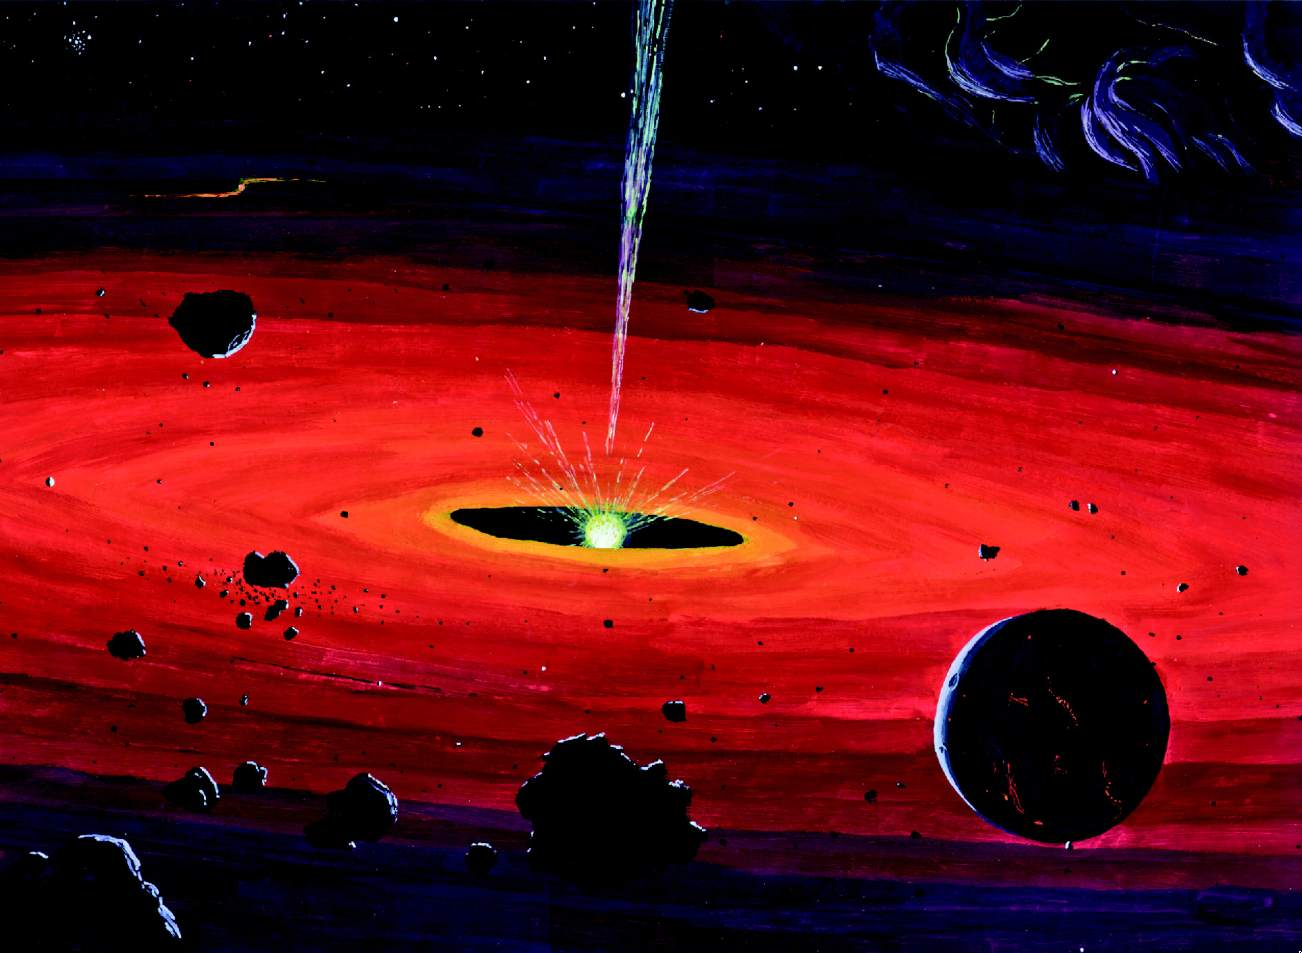
\includegraphics[height=\paperheight]{../obr/fmt.jpg}}%
\begin{frame}
	\textcolor{white}{\textbf{Děkuji za pozornost.}}
\end{frame}
}

\end{document}
